\documentclass[margin=1mm]{standalone}

\input{../../tikz}
\input{../../font}
\input{../../tableau_colors}

\begin{document}

\pagestyle{empty}
\pgfdeclarelayer{background}
\pgfdeclarelayer{foreground}
\pgfsetlayers{background,main,foreground}

%\xdefinecolor{darkgreen}{RGB}{175, 193, 36}
\newcounter{cntShader}
\newcounter{cntRoot}
\setcounter{cntShader}{20}
%\def\couleur{darkgreen}

\begin{tikzpicture}
  \foreach \y in {150}{
    \coordinate (a) at (0,1);
    \coordinate (b) at (0:1); % deg, radius
    \foreach \x in {0,...,\y}{%
      \coordinate (c) at ($(b)!2cm!90:(a)$);
      \node[] at (c) {s};
      \node[circ] at (c) {\y,\textbf{\x}};
      \coordinate (b) at (c);
    }
  }
  %\node[] at (0:1) {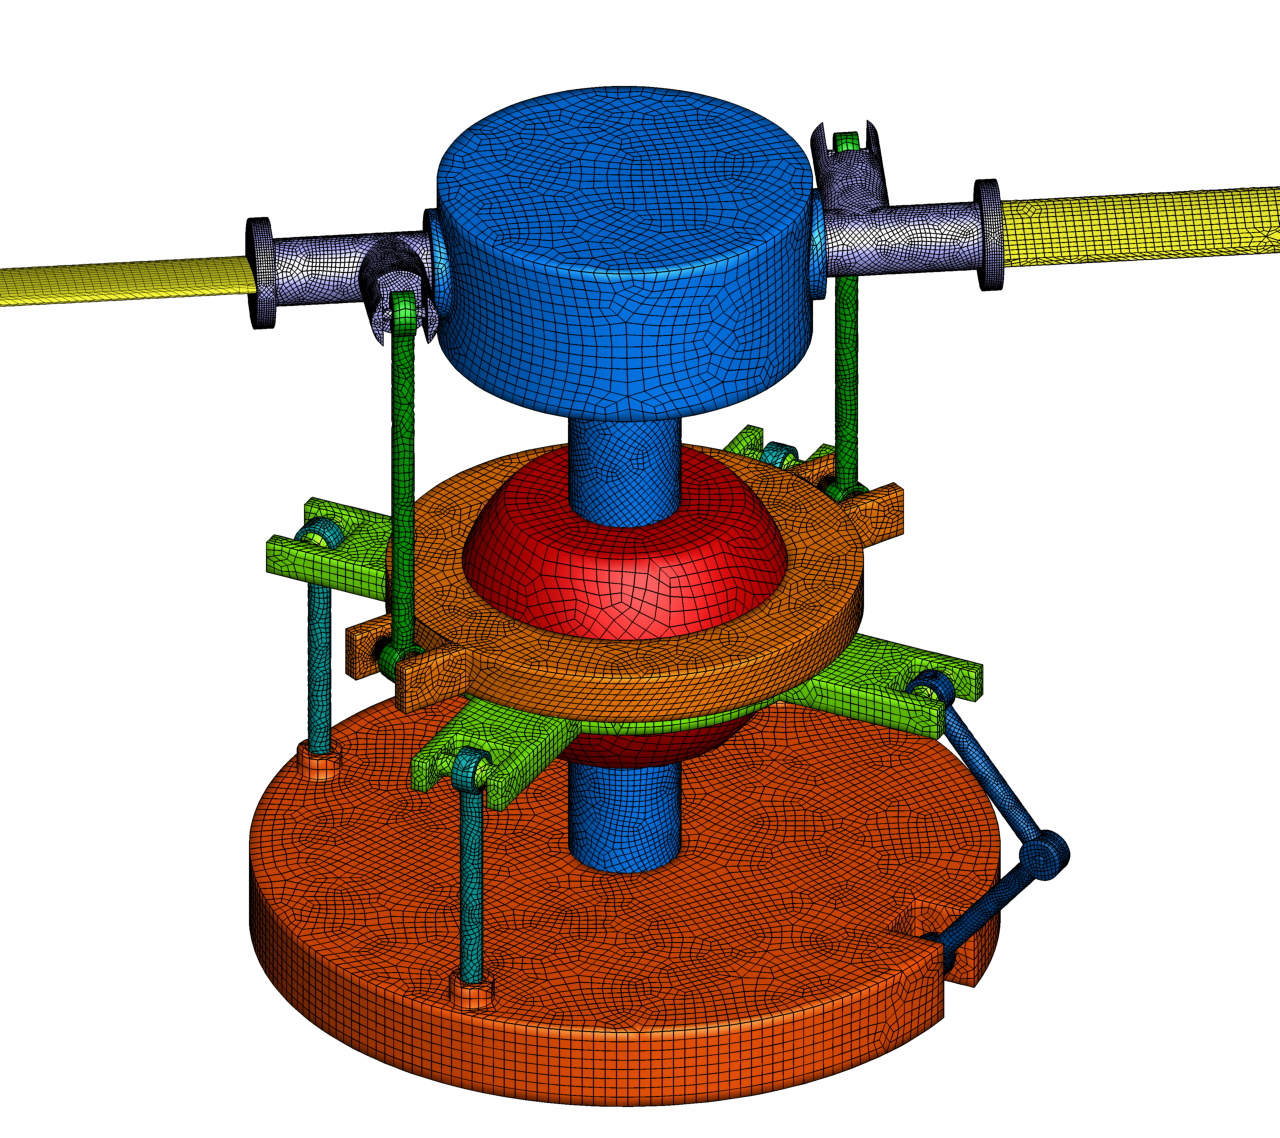
\includegraphics[trim={1pt 1pt 1pt 1pt},clip,width=0.9cm]{assembly_0.png}};
  %\node[circ, fill opacity=0.0, fill=white, text width=0.85cm] at (0:1) {};
  %\node[fill=white,draw,circle,inner sep=0pt,opacity=0.1] at (0:1) {};
\end{tikzpicture}

\end{document} 
